\chapter{Learning from interactions}
\label{chap:rllearning}

The present chapter extends parameter estimation to a reinforcement learning context.  As explained in the first part of this thesis, a reinforcement learning agent learns how to act through trial and error in a given environment.  In our case, the environment is represented by verbal interactions with human users, and the system behaviour to learn corresponds to dialogue policies mapping dialogue states to relevant system responses. 

The optimisation process is in many respects similar to the one outlined in the previous chapter. Bayesian inference remains the basic instrument for updating distributions over the model parameters on account of the collected evidence.  However, the evidence is no longer represented by examples of expert behaviour as in supervised learning. The learning agent instead actively gathers experience through repeated interactions with (real or simulated) users, and receives feedback on its actions in the form of new observations and rewards. The parameter distributions are gradually refined on the basis of this feedback and subsequently used to select the next actions to execute. To minimise the number of parameters, the domain models are structured through probability and utility rules. This structured modelling approach allows the learning agent to  escape the ``curse of dimensionality'' that often characterises dialogue domains. As a consequence, the number of interactions required to reach dialogue policies of high quality can be greatly reduced. 

The chapter is divided in three sections.  After a short survey of the core concepts of Bayesian reinforcement learning in Section \ref{sec:brl}, we expose in Section \ref{sec:rl-ruleparams} our own reinforcement learning approach to the estimation of rule parameters.  More specifically, we present how the parameters of probabilistic rules can be automatically optimised from interactions using either model-based or model-free strategies. Finally, Section \ref{sec:rllearning-experiments} describes a practical experiment conducted in a human-robot interaction domain. The purpose of the experiment was to analyse the learning performance of two alternative formalisations of the transition model, one encoded with standard categorical distributions, and one structured with probabilistic rules. Empirical results on a user simulator show that the rule-structure model is able to converge to optimal parameters -- and hence achieve higher rewards -- in a much shorter time than unstructured representations. 

\section{Bayesian approaches to reinforcement learning}
\label{sec:brl}

Bayesian reinforcement learning has recently emerged as a generic framework for learning and acting in uncertain environments \citep{poupart2008,Ross:2011,brl2012}. As in other types of Bayesian learning methods, one core idea of Bayesian reinforcement learning is to maintain explicit probability distributions over the domain parameters and gradually narrow down the spread of these distributions as more experience is collected. However, reinforcement learning agents are not merely passive observers in an interaction but active participants.  The agent must therefore decide how to act after each turn in order to move the interaction forward. 

As explained in Section \ref{sec:rl}, these actions must balance between exploration (trying out new actions) and exploitation (preferring actions that are most likely to yield higher rewards). Bayesian reinforcement learning can offer principled solutions to the exploration-exploitation dilemma, as model uncertainty is explicitly accounted for in the action selection process \citep{Duff:2002,Ross:2011}.  A Bayesian agent will therefore select actions that are expected to provide the highest long-term return given the current model uncertainty. When this uncertainty is high, information-gathering actions will be preferred since they lead to a better understanding of the environment dynamics and are therefore more likely to yield higher rewards in the future. This inclination to explore will gradually fade away as the learning agent develops a better grasp of its domain and becomes as a result more confident about the relative merits of its own actions.
%\footnote{The representation of this model uncertainty and its inclusion in the action selection process can however take multiple forms \cite[see e.g.][for more details]{brl2012}.}
As for other reinforcement learning methods, Bayesian reinforcement learning can be classified in model-based and model-free approaches. 


\subsubsection*{Model-based methods}

Model-based approaches seek to learn an explicit model of the domain in the form of transition, reward and observation models.  One benefit of model-based approaches is the relative simplicity of parameter estimation, as the model parameters can be directly updated upon the reception of each observation and reward using standard Bayesian inference. The policy optimisation is however more complex, as the policy must be determined in a problem space that combines state uncertainty, stochastic action effects, and uncertainty over the model parameters.  The result is an augmented POMDP where the state also includes random variables expressing the model parameters in addition to traditional state variables. \citep{Duff:2002,Ross:2011}. 

For domains of small to medium size, approximate dynamic programming methods can be applied to generate the $\boldsymbol\alpha$-vectors for this augmented POMDP.  Point-based solvers \citep{Pineau:2004,Porta:2006} have in particular showed reasonable performance on a variety of domains. The multivariate and continuous nature of the parameter variables remains however a major issue. 

An alternative to these offline approaches is online planning.  Online planning selects the optimal action at runtime, during the interaction. Instead of trying to compile a policy for all possible states (as done in dynamic programming), online planning concentrates on selecting the best action for the current state. This selection process is typically implemented in a search tree representing possible actions and their effects in terms of rewards and new observations. This tree is gradually expanded until a given planning horizon is reached.  Several approximate methods have been recently developed, based on e.g. point-based value iterations \citep{ross2008} and Monte Carlo tree search \citep{silver2010uct}. The action leading to the highest return on the search tree is then determined to be the optimal action. Online planning offers many theoretical and practical benefits, such as the possibility to dynamically adapt the domain models at runtime and select actions that reflects this adaptation. As planning is performed at execution time, while the interaction is taking place, it must however meet real-time constraints. 

Interestingly, offline and online approaches to planning are not mutually exclusive, but can be combined together to combine their respective benefits.  The idea is to perform offline planning to precompute a rough policy, and use this policy as a heuristic approximation to guide the search of an online planner \citep{RossC07}. These heuristic approximations can for instance be used to provide lower and upper bounds on the value functions associated with the dialogue states of the search tree.  Based on these bounds, the planning algorithm can concentrate its computational efforts in the most fruitful regions of the search space and quickly discard irrelevant actions. 

\subsubsection*{Model-free methods}

Model-free approaches adopt a different learning strategy and directly estimate a dialogue policy from experience, without seeking to construct explicit internal models of the domain. One simple estimation strategy, formalised by e.g. \cite{Dearden:1998}, is to assign prior distributions to the $Q$-value estimates associated with state-action pairs, and iteratively refine these distributions upon the completion of each action. This update generally relies on Bellman's equation, since the $Q$ values are never directly observed (only the observations and rewards are available to the agent). The optimal action is then simply defined as the one that maximises the $Q$ values for the current state, modulo an ``exploration bonus'' added at learning time to favour exploratory strategies. 

Other Bayesian model-free approaches that are worth mentioning include Gaussian processes to handle problems with continuous state and actions spaces \citep{Engel:2005}, and policy gradient methods, which directly optimise a parametrised policy by gradient ascent without resorting to $Q$ values \citep{bb-ihgbps-01,GhavamzadehE06}.  Policy gradient methods have also been combined with actor-critic methods to reduce the variance of the parameter estimates \citep{Ghavamzadeh:2007}.

Bayesian reinforcement learning has been the subject of much recent research and led to the development of powerful optimisation methods \cite[see e.g.][for a detailed survey]{brl2012}. Scalability remains nevertheless a important concern when porting these methods to real applications.  The number of parameters is in particular an major bottleneck for many learning methods, especially in partially observable domains. We shall see in the next sections how probabilistic rules can help addressing this issue. 

\section{Reinforcement learning of rule parameters}
\label{sec:rl-ruleparams}

Two distinct learning approaches were developed in the course of this thesis to optimise model parameters from interactions. Both employ Bayesian reinforcement learning as theoretical framework and probabilistic rules as representation formalism, but branch out in their choice of optimisation strategies:

\begin{itemize}
\item The first approach follows a model-based strategy.  In this approach, the rule-structured models $\mathcal{M}$ of the domain correspond to transition, observation and reward models. The models are associated to a collection of parameters $\boldsymbol\theta$ with prior distributions $P(\boldsymbol\theta)$.  These parameter distributions are updated on the basis of the observations and rewards received by the system during the interactions. Forward planning is used at runtime to calculate the expected cumulative utilities of possible actions and select the one yielding the maximum utility given the current dialogue state and rule parameters. 

\item The second approach is a model-free strategy.  The transition and reward models are here replaced by  a collection of parametrised utility rules representing the estimated $Q$ value for the system actions. In contrast to the model-based strategy, the utility parameters are here updated via a temporal-difference learning method.  The actions to execute are determined by selecting the action with highest estimated $Q$-value in most cases, and exploring new actions in the remaining cases. 
\end{itemize}

The two sections below flesh out these two approaches in more detail. 

\subsection{Model-based approach}

\subsubsection*{Parameter estimation}

The model-based approach relies on the specification of probabilistic rules that describe:
\begin{itemize}
\item the \textit{transition model} for the domain, i.e. how the dialogue state is likely to change as a result of the system actions
\item the \textit{observation model} for the domain, i.e. what are the likely observations associated with a given dialogue state;
\item the \textit{reward model} for the domain, i.e. what are the immediate utilities (reflecting the system objectives) that result from the execution of particular system actions.
\end{itemize}

Figure \ref{fig:modelbasediagram} depicts a dynamic decision network where transition model is encoded in the figure as a distribution $P(s_t \, | \, s_{t-1}, a_{t-1} \,; \boldsymbol\theta_T)$, the observation model by a distribution $P(o_t \, | \, s_t\,; \boldsymbol\theta_O)$ and the reward model by a distribution $U_{r_t}(s_t,a_t\,; \boldsymbol\theta_R)$.\footnote{The figure naturally offers a simplified picture of the actual graphical model for the domain. In particular, the dialogue states, system actions and observations are all reduced to a single variable.  The figure also abstracts away from the intermediary rule nodes connecting the variables in the network, and upon which the parameters are attached.}

\begin{figure}[h]
\centering
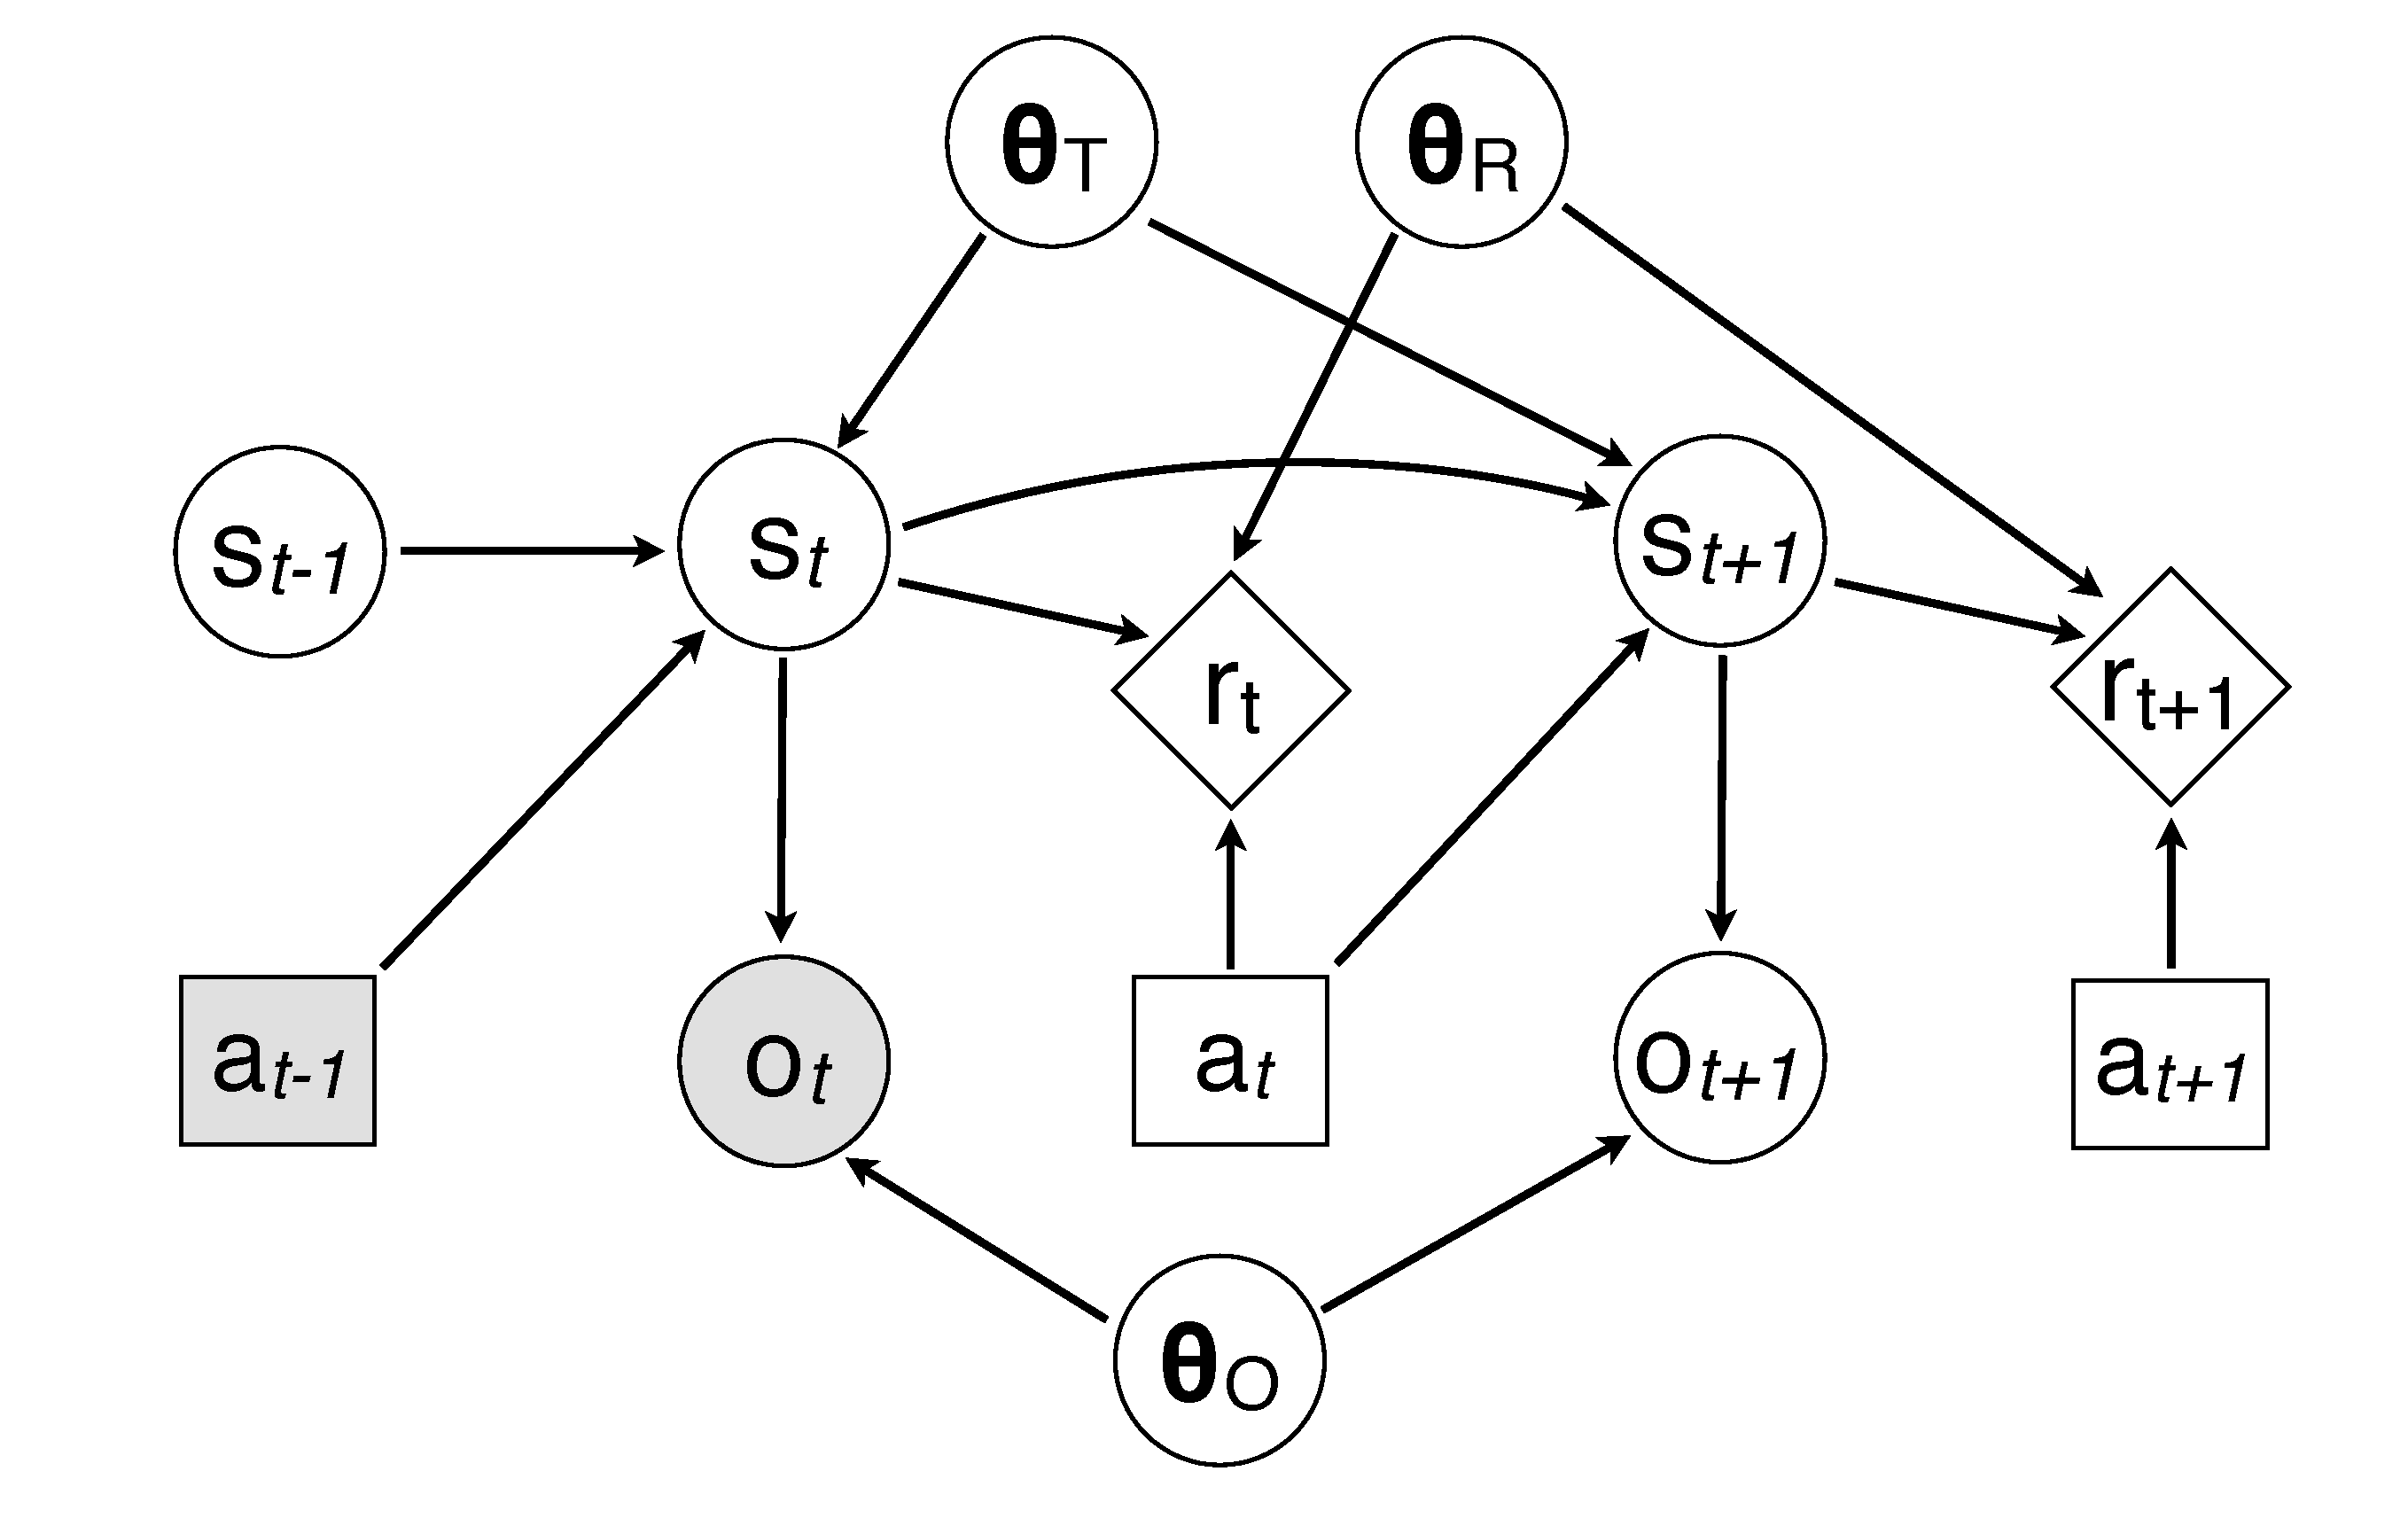
\includegraphics[scale=0.25]{imgs/modelbaseddiagram.pdf}
\caption{Dynamic decision network for a model-based learning strategy expanded on three time steps, with parameters for the transition, observation and reward models.}
\label{fig:modelbasediagram}
\end{figure}

In the worst case learning scenario, the probabilistic rules corresponding to these models all include unknown parameters that must be estimated from data.  Fortunately, this worst case scenario where $\boldsymbol\theta_T$, $\boldsymbol\theta_R$ and $\boldsymbol\theta_O$ must all be learned from scratch rarely happens in practice. As exemplified in the experiment described at the end of this chapter, the reward and observation models can often be defined by the system designer prior to learning. 
%The transition model is typically the domain model that is most difficult to capture, as it expresses the dynamics of the interaction -- i.e. how the user is expected to interact with the system. 

Two types of information sources are available to the agent to refine its parameters during the interaction: the observations and the rewards.  In the model-based setting, parameter update is quite straightforward.  The key idea is to include the parameter variables as part of the dialogue state.  The probability distributions of these parameters are then automatically updated as part of the state update process (see Algorithm \ref{algo:stateupdate} in Section \ref{sec:processing-workflow}). There is therefore no need for special purpose mechanisms beyond standard Bayesian update.

\subsubsection*{Example of parameter update}

Let us illustrate this process on the domain example from Section \ref{sec:detailedexample}.  The example of dialogue snippet remains unchanged:
 \begin{dialogue} 
\speak{User } Now move forward \\ $\phantom{b}$ $\tilde{a}_u = \langle (\mathit{Request(Forward)}, 0.6), (\mathit{Request(Backward)}), 0.4)\rangle$  \\[-3mm]
\speak{System } Could you please repeat? \\[-3mm]
\speak{User } Please move forward! \\ $\phantom{b}$ $\tilde{a}_u = \langle (\mathit{Request(Forward)}, 0.7), (\mathit{Other}, 0.2), (\mathit{Request(Backward)}, 0.1) \rangle$ \\[-4mm]
\end{dialogue}

We shall however assume that the effect distribution associated with the predictive rule $r_{11}$ is unknown and replaced by parameters: 
\begin{align*}
r_{11}: \ \ & \forall y: \\ 
& \textbf{if} \ (a_m = \mathit{AskRepeat} \land a_u=y) \ \textbf{then} \\ 
& \; \;  \begin{cases} 
P(a_{u\mbox{-}p} = y) = \theta_{r_{11}(1,1)} \\ 
P([\cdot]) = \theta_{r_{11}(1,2)} \\ 
\end{cases}
\end{align*}
In order to estimate these parameters through Bayesian inference, we first define a prior probability distribution for the two-dimensional parameter $\boldsymbol\theta_{r_{11}(1,\cdot)}$.  We shall chose in this example to represent the distribution $P(\boldsymbol\theta_{r_{11}(1,\cdot)}$ to be $\sim \mathrm{Dirichlet}(2,1)$, since can reasonably presuppose that the user is more likely than not to repeat her/his last utterance after an explicit request from the system.

Figure \ref{fig:learningexample} shows how the distribution over the parameter values for $\boldsymbol\theta_{r_{11}(1,\cdot)}$ is automatically refined as part of the state update operation.  For simplicity's sake, the figure ignores the steps related to action selection and concentrates on the application of rule $r_{11}$.  The first step illustrates the instantiation of the rule along with its parameter. Upon the reception of a new observation in the form of a user input $a_u'$, the dialogue state and parameters are updated (step 2). After pruning and integration of the evidence (step 3), we notice that the parameter distribution $P(\boldsymbol\theta_{r_{11}(1,\cdot)})$ has shifted part of its probability mass further to the right. In other words, the probability of the user following the system request becomes somewhat more likely. The posterior distribution $P(\boldsymbol\theta_{r_{11}(1,\cdot)})$ following the update is constructed using kernel density estimation. 

\begin{figure}[h]
\centering
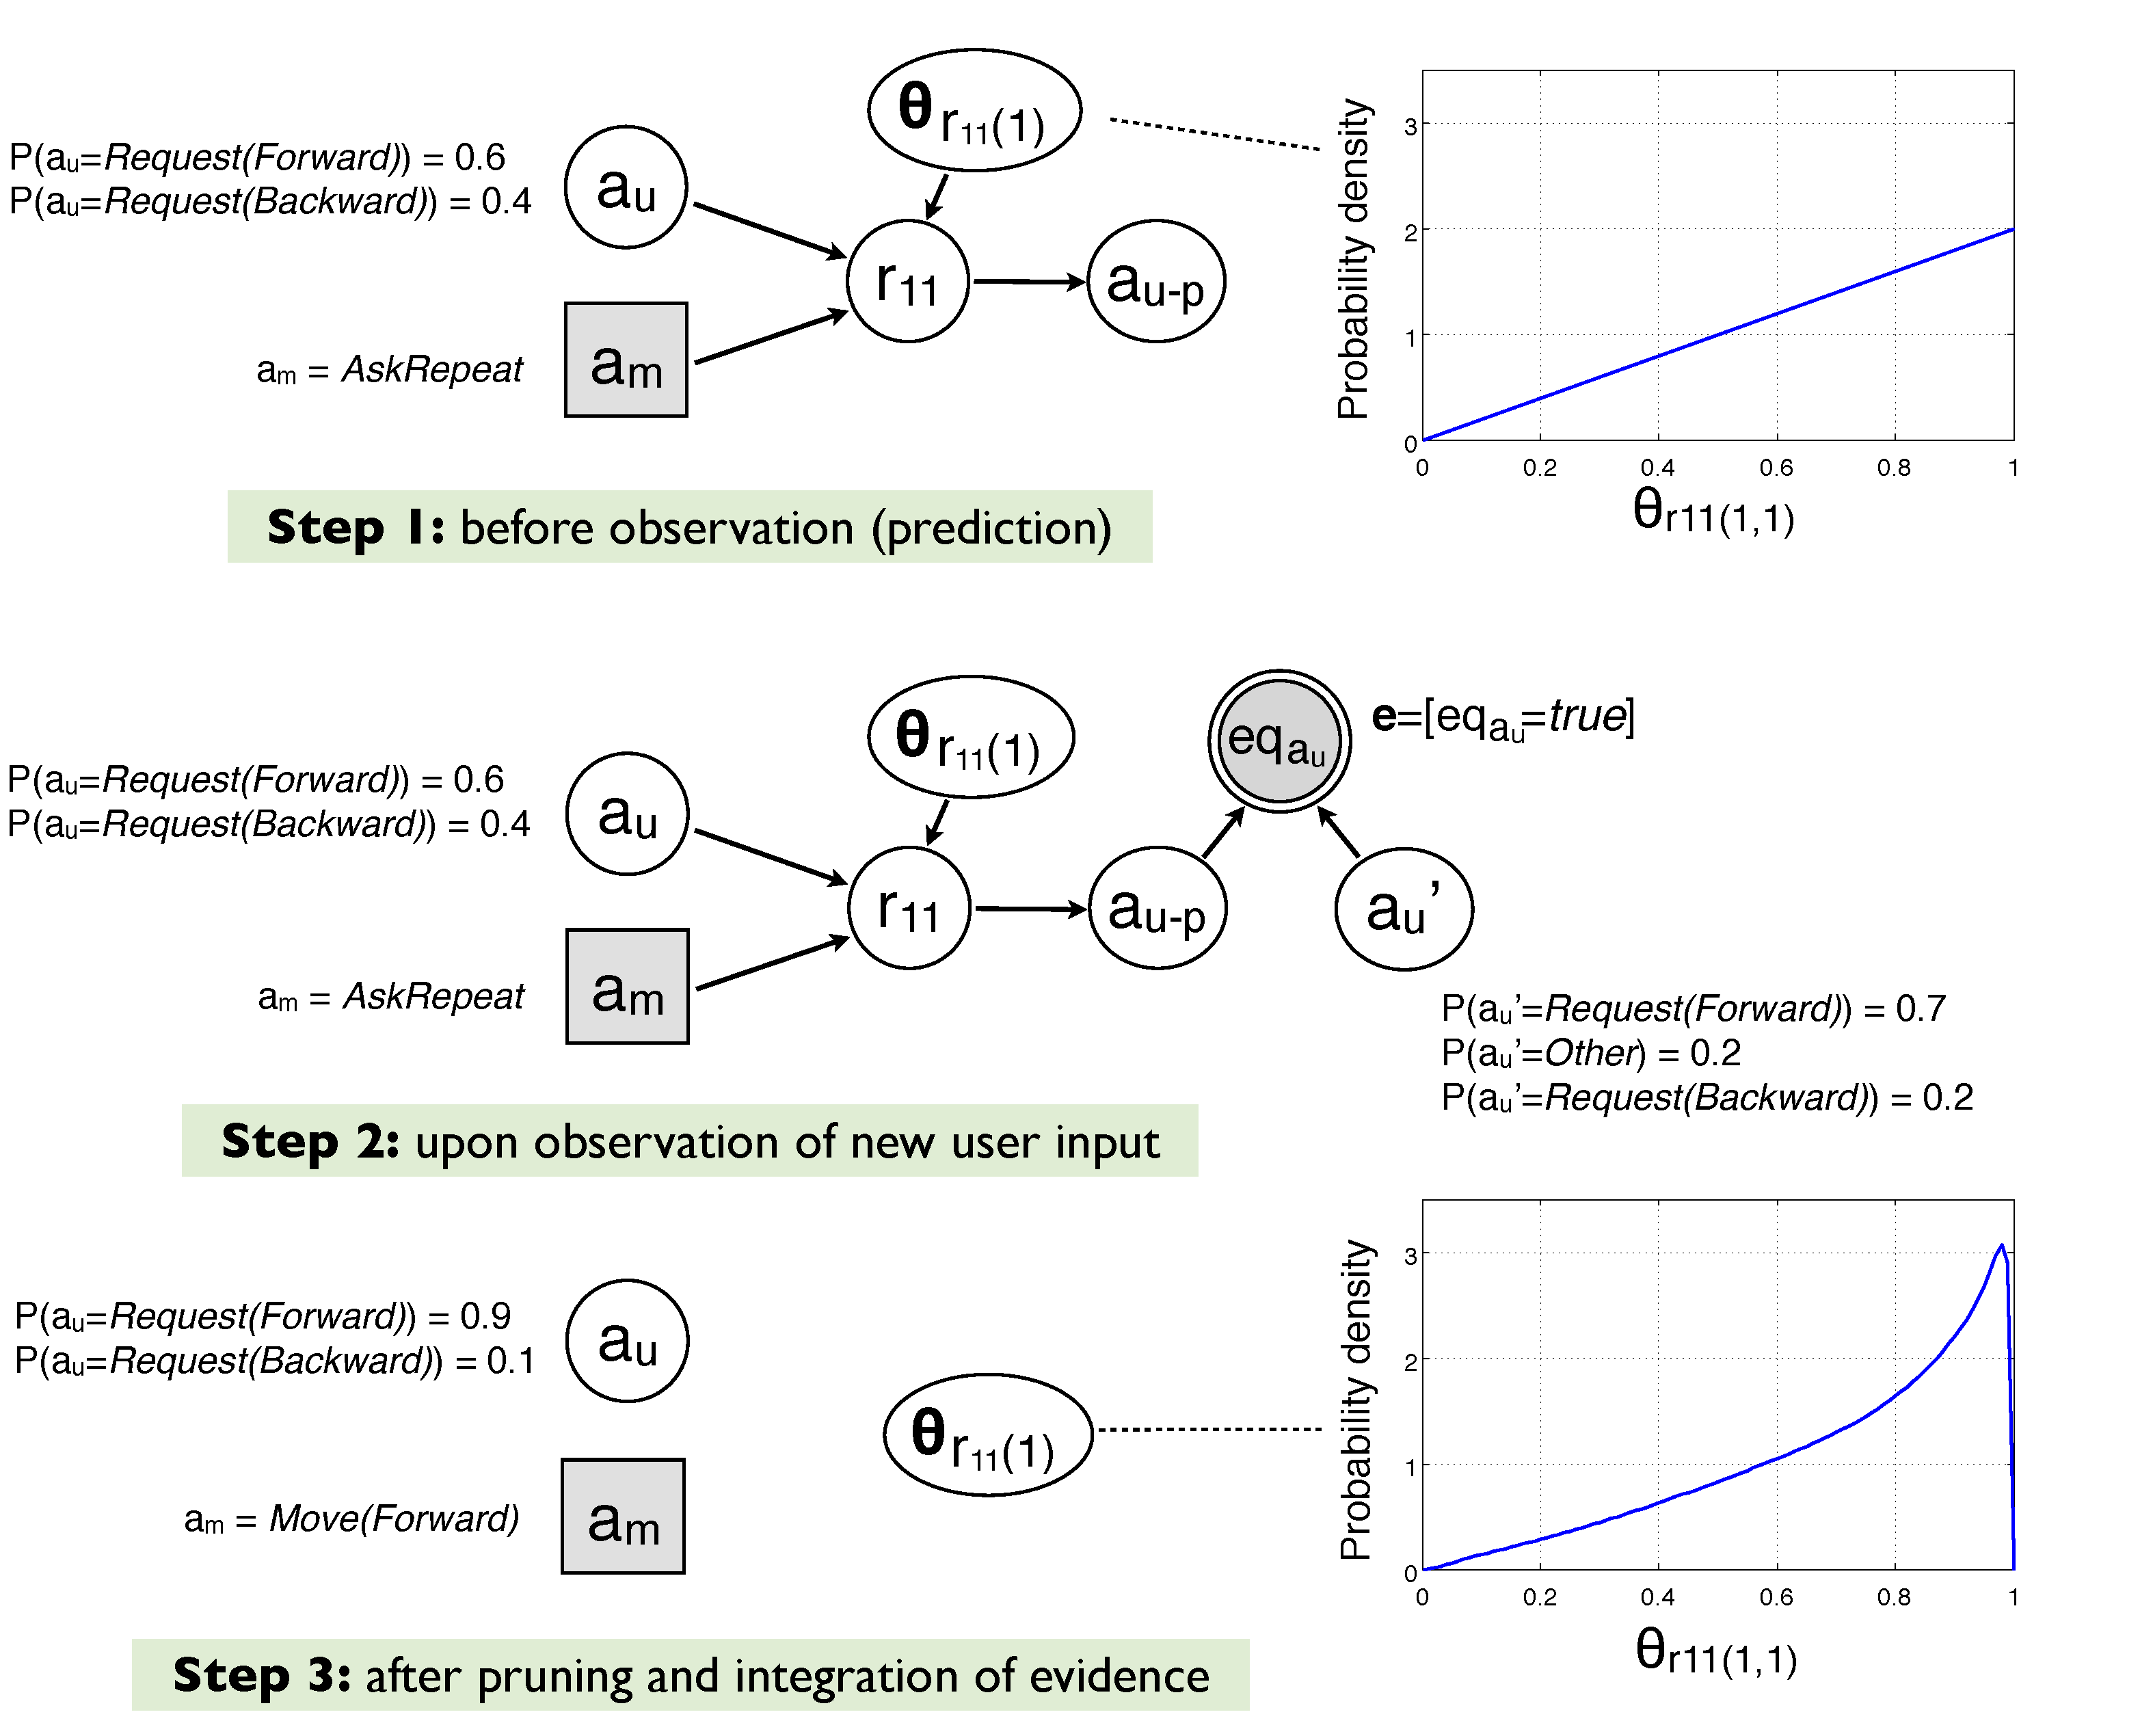
\includegraphics[scale=0.30]{imgs/learningexample.pdf}
\caption{Parameter update for $\boldsymbol\theta_{r_{11}(1,\cdot)}$ after the reception of a new user input. }
\label{fig:learningexample}
\end{figure}


\subsubsection*{Action selection}

 As the $Q$ values are no directly accessible in model-based approaches, action selection must resort to either dynamic programming or forward planning to calculate the expected future rewards of each action.  This planning step is the computational bottleneck in model-based Bayesian reinforcement learning, since the agent needs to reason not only over all the current and future states, but also over all possible models (parametrised by the $\boldsymbol\theta$ variables).  The high dimensionality of the task often prevents the use of offline solution techniques. We apply in this work a simple forward planning algorithm coupled with importance sampling. 

Algorithm \ref{algo:planning} selects the action to execute through forward planning on a given horizon $h$.  The selection procedure relies on the recursive function \textsc{Calculate-Q-Values}() to compute the Q-values of possible actions. The $Q$ value of an action is the discounted addition of its immediate reward (line 3 in Algorithm \ref{algo:qval}) and the expected future reward following its execution.  Line 6 loops on possible observations.  For efficiency reasons, only a limited number of high-probability observations are sampled. For each selected observation, the dialogue state is updated and its maximum expected reward is computed.  The procedure stops when the planning horizon has been reached, or the algorithm has run out of time. The planner then simply selects the action with maximum expected cumulative utility. 

\begin{algorithm}[h!]
\caption{: \textsc{SelectAction} ($\mathcal{B}, \mathbf{e}$, h)}
\begin{algorithmic}[1] \vspace{1mm}
\REQUIRE Dialogue state $\mathcal{B}$ as a decision network
\REQUIRE Evidence $\mathbf{e}$
\REQUIRE Planning horizon $h$
\ENSURE Selected action $\mathbf{a}^*$
\STATE $Q_{\mathcal{B}} \leftarrow $ \textsc{Calculate-Q-Values} ($\mathcal{B}, \mathbf{e}, h)$
\STATE Find optimal value $\mathbf{a}^* = \argmax_{\mathbf{a}} Q_{\mathcal{B}}(a)$
\STATE Remove utility nodes from the state $\mathcal{B}$
\RETURN $\mathbf{a}^*$
\end{algorithmic}
\label{algo:planning}
\end{algorithm}


\begin{algorithm}[h!]
\caption{: \textsc{Calculate-Q-Values} ($\mathcal{B}, \mathbf{e}, h)$}
\begin{algorithmic}[1] \vspace{1mm}
\STATE Let $\mathbf{A}$ be the set of all decision variables in $\mathcal{B}$
\FORALL {possible action $\mathbf{a} \in Val(\mathbf{A})$}
\STATE $Q_{\mathcal{B}}(a) \leftarrow U_{\mathcal{B}}(\mathbf{a}, \mathbf{e})$
\IF {$h > 1$}
\STATE $\mathcal{B}' \leftarrow $ dialogue state updated from $\mathcal{B}$ after action $\mathbf{a}$
\FORALL {possible observation $\mathbf{o}$}
\STATE $\mathcal{B} \leftarrow $ dialogue state updated from $\mathcal{B}'$ after observation $o$
\STATE $Q_{\mathcal{B}''} \leftarrow $ \textsc{Calculate-Q-Values}($\mathcal{B}'', \mathbf{e}, h\mbox{-}1$)
\STATE $Q_{\mathcal{B}}(a) \leftarrow Q_{\mathcal{B}}(a) + \gamma \ P_{\mathcal{B}'}(\mathbf{o}) \ \max_{\mathbf{a}'} Q_{\mathcal{B}''}(\mathbf{a}')$
\ENDFOR
\ENDIF
\ENDFOR
\RETURN $Q_{\mathcal{B}}$
\end{algorithmic} 
\label{algo:qval}
\end{algorithm}

Algorithm \ref{algo:qval} contains two loops: one cycling over the possible actions, and one cycling over the possible observations following the system action. This process can be represented in an AND-OR search tree anchored in the current state. The OR branches denote the system actions and their respective rewards, while the AND branches denote the observations weighted by their likelihood. An example of such search tree is provided in Figure \ref{fig:modelbasediagram} (modified from \cite{ross2008}).


\begin{figure}[h!]
\centering
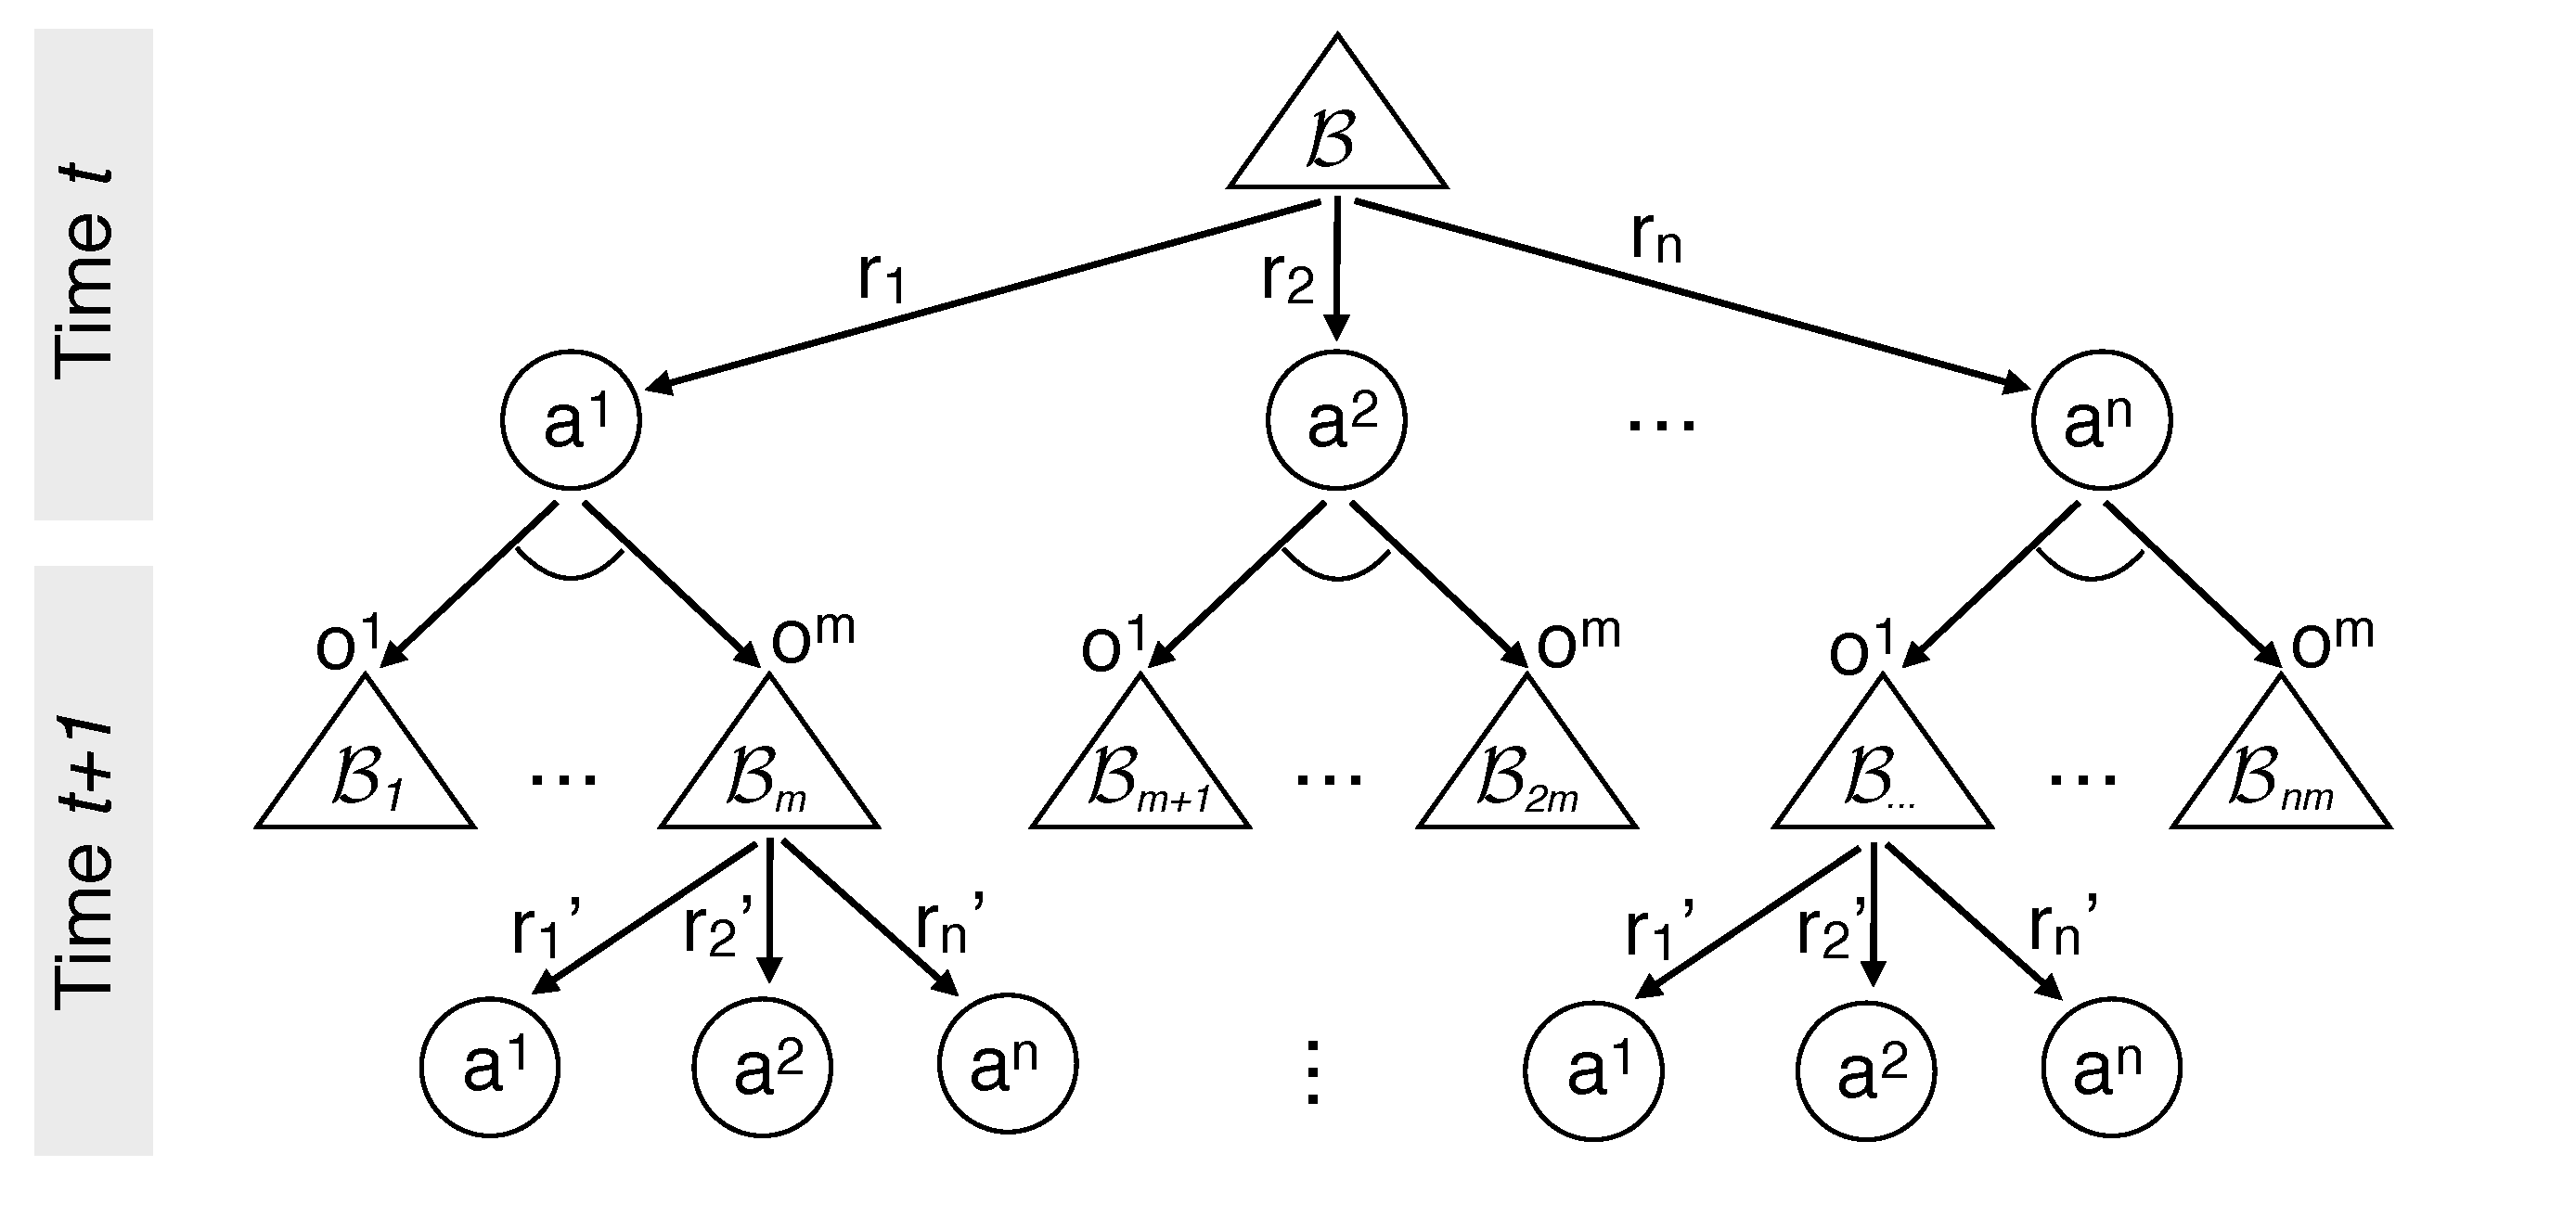
\includegraphics[scale=0.30]{imgs/andortree.pdf}
\caption{AND-OR search tree constructed through forward planning for a horizon of 2.}
\label{fig:modelbasediagram}
\end{figure}

As argued in \cite{onlineplanning-iwsds2012}, the reliance on utility rules to encode the reward model can greatly enhance the tractability of the planning process.  In addition to assigning utilities to system actions, utility rules also implicitly define the set of action values that are relevant at a given time.\footnote{Recall that in Algorithm \ref{algo:instantiateUtilRule} from Section \ref{sec:ruleinstantiation}, the set of possible values of an action node is directly derived from the values listed in the utility nodes connected to it.} In other words, actions that are not deemed relevant in a particular state are automatically filtered out.  Instead of searching through the whole space of possible actions, the planning algorithm is thus limited a subset of actions that are locally relevant.  One interesting aspect of this approach is that the filtering of relevant actions is done solely on the basis of the provided reward model and does not require the integration of additional constraints or ad-hoc mechanisms. This stands in contrast with most existing work in dialogue management, where constraints on possible actions are typically enforced through external filtering techniques defined on the basis of e.g. information-state rules \citep{heeman2007}, finite-state automata \citep{williams2008} or -- in our own previous work on this question -- constraints encoded in Markov Logic \citep{srw-acl2010}. 

 
\subsubsection*{Learning cycle}

The model-based learning cycle is detailed in Algorithm \ref{algo:rlearning_mb}. The learning agent incrementally updates its model parameters $\boldsymbol\theta$  by running a number of interactions, either with a real user or in simulation. Starting with an initial dialogue state, the interaction alternates between the reception of new observations (in the form of e.g. user inputs or contextual changes in the environment) and the execution of system actions following these observations.  The dialogue state is updated after each observation (line 5), using the procedure outlined in Section \ref{sec:processing-workflow}, with the action selection method replaced by Algorithm \ref{algo:planning}. If non-empty actions are selected as a result, those are executed (line 7).   In case the reward model is unknown, the reward resulting from the system actions can be integrated in the set of observations and used to update the reward parameters accordingly. 

\begin{algorithm}[h]
\caption{: \textsc{Model-based-RL-learning} ($\mathcal{M}, \mathcal{B}_0, \boldsymbol\theta, N$)}
\begin{algorithmic}[1]\vspace{1mm}
\REQUIRE Rule-structured models $\mathcal{M}$ for the domain
\REQUIRE Initial dialogue state $\mathcal{B}_0$
\REQUIRE Model parameters $\boldsymbol\theta$ with prior distribution $P(\boldsymbol\theta)$
\REQUIRE Number $N$ of interactions to collect
\ENSURE Posterior distribution $P(\boldsymbol\theta)$ for the parameters  \vspace{1mm}
\FOR {$i = 0 \to N$}
\STATE Start new interaction with initial state $\mathcal{B} = \mathcal{B}_0 \cup \boldsymbol\theta $
\WHILE {interaction is active}
\STATE Get new observations $\mathbf{O}$
\STATE \textsc{UpdateState}($\mathcal{B}, \mathbf{O}$)
\IF {newly selected action $a$ in $\mathcal{B}$}
\STATE Execute action $a$ and get resulting reward $r$
\ENDIF
\ENDWHILE
\ENDFOR
\RETURN $P(\boldsymbol\theta)$
\end{algorithmic} 
\label{algo:rlearning_mb}
\end{algorithm}



\subsection{Model-free approach}

\subsubsection*{Parameter estimation}

In parallel to the model-based learning strategy described above, we also developed a simple Bayesian model-free approach to the estimation of rule parameters.  In this approach, the core model that is to be estimated is the \textit{action-value model} which specifies the expected cumulative reward $Q$ of the system actions depending on the current state. In addition to this action-value model, the domain may also include transition and observation models. It should be however noted that, in model-free approaches, the transition and observation models are only used for state update (if the dialogue state contains state variables that are indirectly inferred from observations, such as the user intentions) and are not exploited in the action selection.  This stands in contrast with model-based approaches to reinforcement learning where transition and observation  models are directly employed to plan the next action.

\begin{wrapfigure}[17]{r}{60mm}
\vspace{-2mm}
\centering
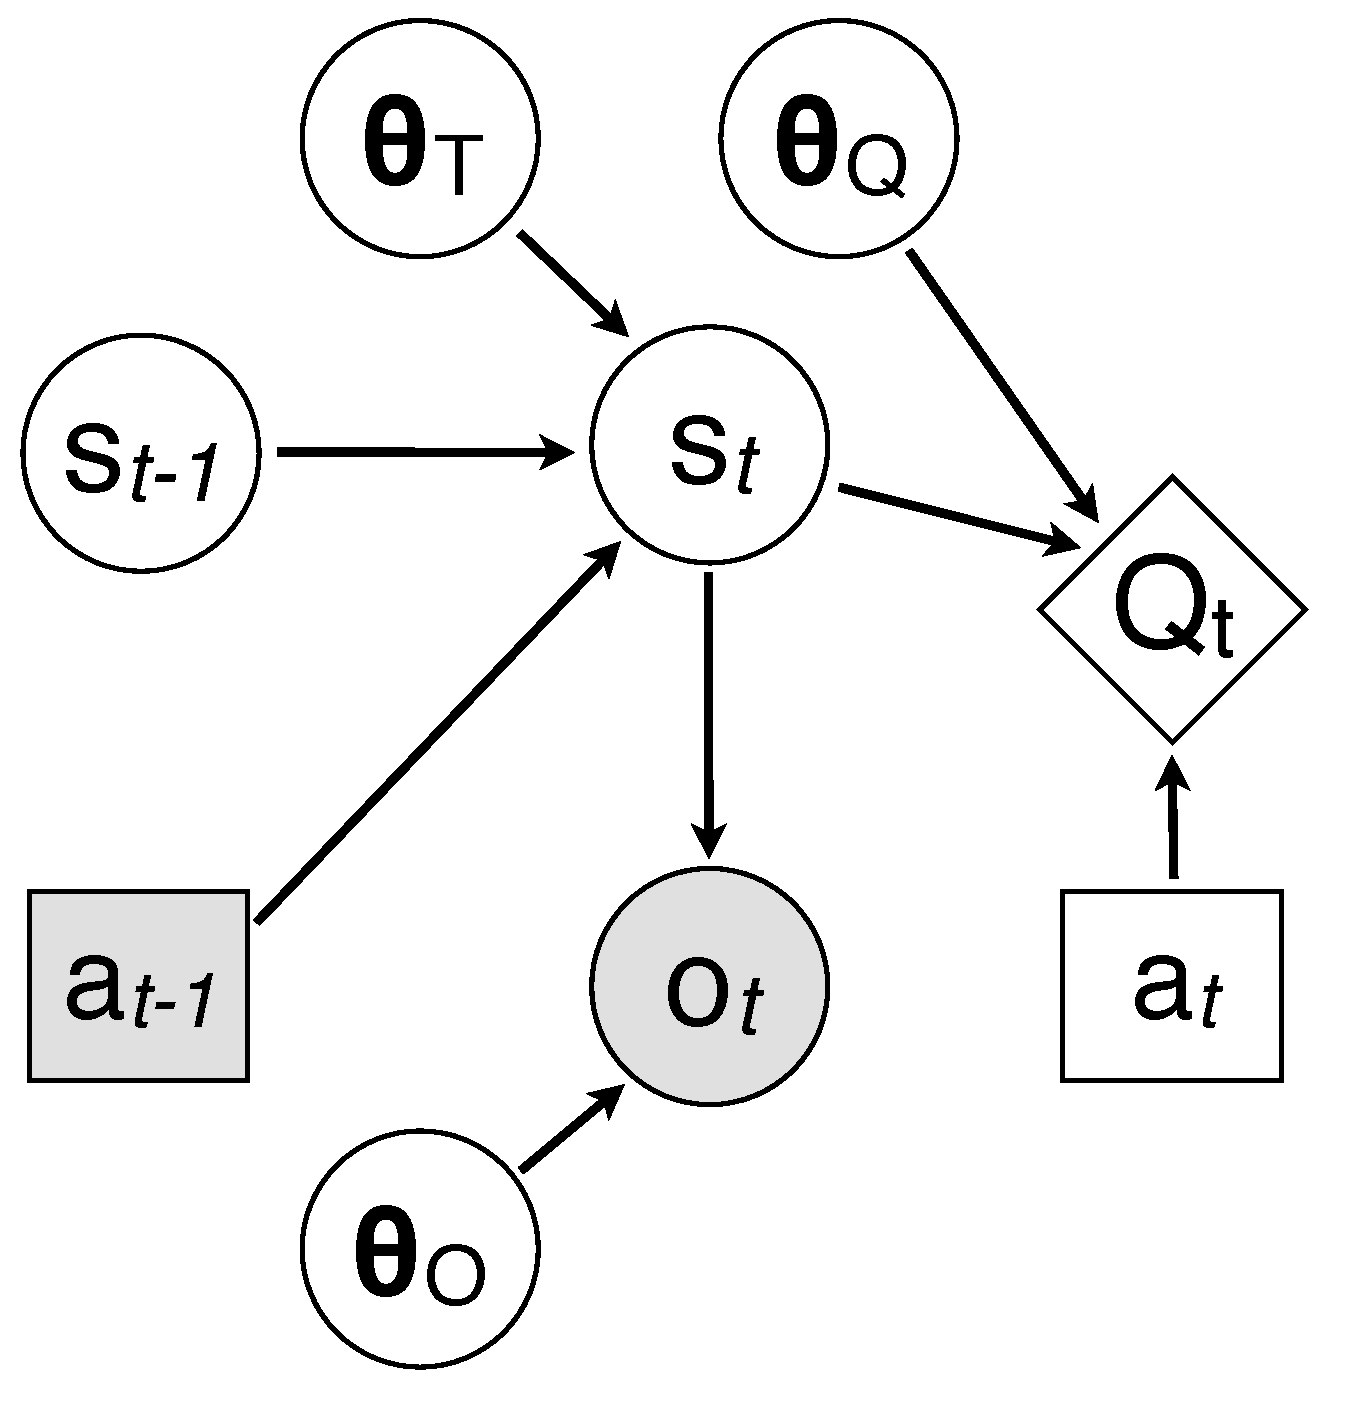
\includegraphics[scale=0.25]{imgs/modelfreediagram.pdf}
\vspace{-2mm}
\caption{Dynamic decision network for a model-free strategy with parameters for the transition, observation and action value models.}
\label{fig:modelfreediagram}
\end{wrapfigure}

As for the model-based approach, all domain models are specified with probabilistic rules. The transition and observation models can be encoded by probability rules, and the $Q$-value by utility rules. In the worst case, all models may include unknown parameters.  The transition model is thus defined as a probability distribution $P(s_t \, | \, s_{t-1}, a_{t-1} \,; \boldsymbol\theta_T)$, the observation model by a distribution $P(o_t \, | \, s_t\,; \boldsymbol\theta_O)$ and the $Q$-value model by a distribution $U_{r_t}(s_t,a_t\,; \boldsymbol\theta_Q)$.  Figure \ref{fig:modelfreediagram} illustrates how these distributions combine to form a dynamic decision network. 

When present, the transition and observation models can be estimated in the same manner as in the model-based approach -- that is, by including the parameters in the dialogue state and refining their distributions as part of the state update process. 

\subsubsection*{Temporal-difference learning}


The estimation of the action-value model is however slightly more intricate, since the $Q$ values are not directly accessible to the learning agent.  The only feedback perceived by the agent is indeed the immediate reward, not the expected cumulative reward $Q$.  One solution is to rely on Bellman's equation to incrementally improve the action-value estimates on the basis of the rewards resulting from the agent actions. Such methods are called temporal-difference methods and regroup popular reinforcement learning algorithms such as SARSA and Q-learning \citep{citeulike:112017}. Temporal-difference methods are also called ``boostrapping'' methods as they approximates new $Q$ value estimates based on previously learned estimates.

The particular model-free learning method applied in this work is based on the well-known SARSA algorithm.\footnote{SARSA stands for State-Action-Reward-State-Action, which is a reference to the processing order of the algorithm.} The classical, MDP-based definition of SARSA proceeds as follows. Let $s_t$ be a dialogue state at time $t$, followed by a system action $a_t$. The execution of the system action $a_t$ results in a reward $r_{t+1}$ and a new dialogue state $s_{t+1}$ which is itself followed by a second system action $a_{t+1}$.  The SARSA update of the $Q$ value estimate for the first action $a_t$ is:
\begin{equation}
Q(s_t, a_t) \leftarrow Q(s_t,a_t) + \alpha \left[r_{t+1} + \gamma \ Q(s_{t+1}, a_{t+1}) - Q(s_t, a_t) \right] 
\end{equation}
where $\alpha$ represents the learning rate of the algorithm. The estimate $Q(s_t, a_t)$ is thus modified in direction of the value $ \left[r_{t+1} + \gamma \ Q(s_{t+1}, a_{t+1} \right]$, with a learning step expressed by $\alpha$. 

%As shown by e.g. \cite{Dearden:1998}, temporal-difference methods are easily amenable to a Bayesian treatment. 

The approach developed in this thesis rests on a simple Baysesian extension of SARSA.  The posterior distribution over the parameters is here computed on the basis of the evidence provided by the reward $r_{t+1}$ and next system action $a_{t+1}$.  Given a sequence of state-action-rewards $\langle \mathcal{B}_t, a_t, r_{t+1}, \mathcal{B}_{t+1}, a_{t+1} \rangle$, we define the likelihood distribution $P(r_{t+1}, a_{t+1} \,; \boldsymbol\theta)$ as:
\begin{equation}
P(r_{t+1}, a_{t+1} \,; \boldsymbol\theta) = \phi \left(\alpha \left[ U_{\mathcal{B}_t}\left(a_t \,; \boldsymbol\theta\right) - r_{t+1} - \gamma \ U_{\mathcal{B}_{t+1}} \left(a_{t+1} \,; \boldsymbol\theta\right) \right] \right) \label{eq:modelfreelikelihood}
\end{equation}
where $\phi(\cdot)$ is the density function for the standard normal distribution $\mathcal{N}(0, 1)$. The standard normal distribution has its peak around the value 0 and decreases exponentially with the distance to this mean. The likelihood distribution will therefore yield a high probability when the initial estimate 
$U_{\mathcal{B}_t}(a_t \,; \boldsymbol\theta)$ available at time $t$ is close to the updated estimate $\left[r_{t+1} + \gamma \ U_{\mathcal{B}_{t+1}} (a_{t+1} \,; \boldsymbol\theta) \right]$ at time $t+1$, and a low probability otherwise. The learning rate $\alpha$ controls the relative weight of this distance between estimates. 

Based on the likelihood distribution defined in Equation \eqref{eq:modelfreelikelihood}, the posterior distribution on the parameters is finally rewritten as: 
\begin{equation}
P(\boldsymbol\theta \, | \, r_{t+1}, a_{t+1}) = \eta \ P(r_{t+1}, a_{t+1} \,; \boldsymbol\theta)  \ P(\boldsymbol\theta)  \label{eq:posteriormodelfree}
\end{equation}


\subsubsection*{Action selection}

The above section described how the parameter distributions were updated on the basis of the received rewards and executed actions, but did not explain how the system actions were selected at runtime.  A simple strategy is to select the action yielding the maximum $Q$ value for the current state.  This greedy strategy can however result in poor control policies if the agent gets stuck in a suboptimal behaviour.  Greedy strategies can be improved by allowing the agent to explore other actions once in a while. The relative frequency of these exploration actions compared to the  ``greedy'' actions is expressed by the probability $\epsilon$, which is usually small. This method is called an $\epsilon$-greedy strategy and is illustrated in Algorithm \ref{algo:egreedy}.

\begin{algorithm}[h!]
\caption{: \textsc{SelectAction} ($\mathcal{B}, \mathbf{e}$)}
\begin{algorithmic}[1] \vspace{1mm}
\REQUIRE Dialogue state $\mathcal{B}$ as a decision network
\REQUIRE Evidence $\mathbf{e}$
\ENSURE Selected action $\mathbf{a}^*$
\STATE Select value $\mathbf{a}^* = \begin{cases} \argmax_{\mathbf{a}} U(\mathbf{a}, \mathbf{e}) & \text{with probability } (1- \epsilon) \\ \text{another action} & \text{with probability } \epsilon \end{cases}$
\STATE Remove utility nodes from the state $\mathcal{B}$
\RETURN $\mathbf{a}^*$
\end{algorithmic}
\label{algo:egreedy}
\end{algorithm}

\subsubsection*{Learning cycle}

The model-free learning cycle is mostly similar to the one defined in the model-based setting.  As shown in Algorithm \ref{algo:rllearning_modelfree}, the agent estimates the values of its rule parameters by collecting a number of interactions.  Each interaction starts from the initial dialogue state $\mathcal{B}_0$ and unfolds as a sequence of observations and actions.  The dialogue state contains both traditional state variables and parameter variables.  After perceiving new observations, the dialogue state is correspondingly updated -- including transition and observation parameters if present in the domain (line 5).  The update process comprises the selection of new system actions, according to the $\epsilon$-greedy selection procedure shown in Algorithm \ref{algo:egreedy}. When a new action is selected, the posterior distributions over parameters are correspondingly updated through temporal-difference learning (line 7).\footnote{This operation can only proceed when the selected action follows another system action in the interaction.} The action is then executed and the resulting reward is retrieved (line 8).  The process is repeated for each interaction. 


\begin{algorithm}[h]
\caption{\textsc{Model-free-RL-learning} ($\mathcal{M}, \mathcal{B}_0, \boldsymbol\theta, N$)}
\begin{algorithmic}[1]\vspace{1mm}
\REQUIRE Rule-structured models $\mathcal{M}$ for the domain
\REQUIRE Initial dialogue state $\mathcal{B}_0$
\REQUIRE Model parameters $\boldsymbol\theta$ with prior distribution $P(\boldsymbol\theta)$
\REQUIRE Number $N$ of interactions to collect
\ENSURE Posterior distribution $P(\boldsymbol\theta)$ for the parameters  \vspace{1mm}
\FOR {$i = 0 \to N$}
\STATE Start new interaction with initial state $\mathcal{B} = \mathcal{B}_0 \cup \boldsymbol\theta $
\WHILE {interaction is active}
\STATE Get new observations $\mathbf{O}$
\STATE \textsc{UpdateState}($\mathcal{B}, \mathbf{O}$)
\IF {newly selected action $a$ in $\mathcal{B}$}
\STATE Update posterior $P(\boldsymbol\theta \, | \, r, a)$ based on Eq. \eqref{eq:posteriormodelfree}
\STATE Execute action $a$ and get resulting reward $r$
\ENDIF
\ENDWHILE
\ENDFOR
\RETURN $P(\boldsymbol\theta)$
\end{algorithmic} 
\label{algo:rllearning_modelfree}
\end{algorithm}


\section{Experiments}

\label{sec:rllearning-experiments}

\note{bla bla }


\subsection{Wizard-of-Oz data collection}

\subsection{User simulator}

\subsection{Experimental setup}

\subsection{Empirical results}

\subsection{Analysis}


\section{Conclusion}

As in other areas of machine learning, Bayesian techniques are increasingly popular in reinforcement learning.
